\subsection{DNA structure \label{secStructure}}

In this paper, we follow the approach of Knotts, De Pablo \etal \cite{knotts2007coarse} to model the structure of B-DNA. In Figure \ref{dna_forms}, the main three structural forms of DNA are illustrated.

\begin{figure}[htbp]
\begin{center}
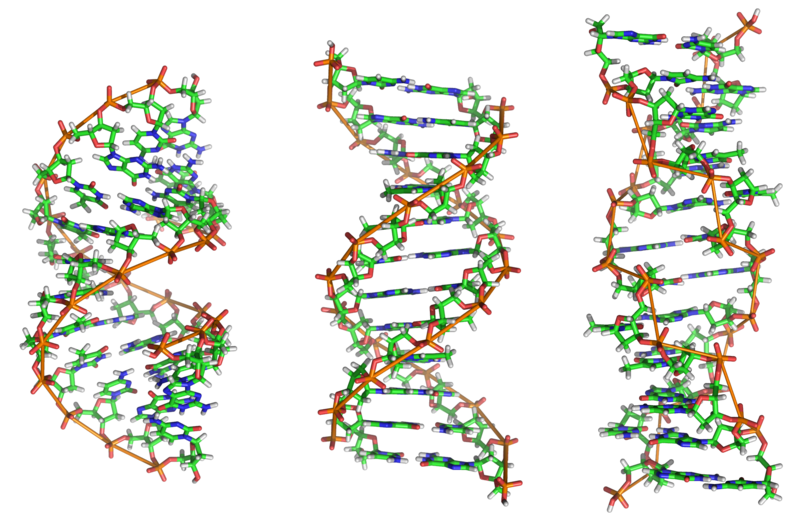
\includegraphics[width=14cm]{images/dna_forms.png}
\caption{Structural forms of DNA: A-DNA (left), B-DNA (center) and Z-DNA (right). Figure from \href{http://www.molecularstation.com}{molecularstation.com}.}
\label{dna_forms}
\end{center}
\end{figure}


The algorithm to build up a single strand is to follow the screw symmetry of B-DNA by placing consecutive monomers on the $z$-axis of space (separated by an axial rise of $3.38$\,\Angstrom), and rotating each consecutive monomer by an angle of $36$ degrees. In practice, this means that if a monomer is placed at location $(r, \phi, z)$, the consecutive monomer on the same strand is placed at $(r, \phi + 36\degree, z + 3.38\,\text{\Angstrom})$. To build up the complementary strand (yielding the characteristic double stranded helical structure of DNA), an atom at $(x, y, z)$ on the first strands has its complementary atom on the other strand at $(x, -y, -z)$ with the $x$-axis taken orthogonal to the helical axis and always along the line connecting the complementary bases of the complementary monomers (i.e. the $x$-axis also rotates $36\degree$ along the $z$-axis for consecutive base pairs along the double strand).

Knotts \etal \cite{knotts2007coarse} used the DNA molecular data of ref. \cite{crcBiochem1976}, and averaged positions for each of the three sites per nucleus yielding the data in table \ref{dnaStructureData}. Schematically, this structure yields the major and minor grooves as illustrated in Figure \ref{schematic_knotts}. The phosphate and sugar sites on the backbone of the molecule are placed at the centers of mass of the molecules; and to map the location of the hydrogen bonds the bases Ab and Gb are placed at the N1 position of the B-DNA isoform; bases Tb and Cb at the N3 position. 

\begin{table}[htdp]
\caption{Structural data for B-DNA helices, calculated by Knotts \etal \cite{knotts2007coarse}.}
\begin{center} \footnotesize
\begin{tabular}{|l|rrrrc|c|}
\hline
 &\ \  $x$ (\Angstrom)\ \ &\ \  $y$ (\Angstrom)\ \  &\ \  $z$ (\Angstrom)\ \  &\ \  $r$ (\Angstrom)\ \  &\ \  $\phi$ (degrees)\ \  & \ \ Mass (amu) \\
\hline
Phosphate (P) & -0.628 & 8.896 & 2.186 & 8.918 & 94.038 & 94.97 \\
Sugar (S) & 2.365 & 6.568 & 1.280 & 6.981 & 70.197 & 83.11 \\
Adenine base (Ab) & 0.575 & 0.516 & 0.051 & 0.773 & 41.905 & 134.1\\
Thymine base (Tb) & 0.159 & 2.344 & 0.191 & 2.349 & 86.119 & 125.1\\
Cytosine base (Cb) & 0.199 & 2.287 & 0.187 & 2.296 & 85.027 & 110.1\\
Guanine base (Gb) & 0.628 & 0.540 & 0.053 & 0.828 & 40.691 & 150.1\\
\hline
\end{tabular}
\end{center}
\label{dnaStructureData}
\end{table}%


At the beginning of the simulations, the world gets filled with a centered DNA helix of a given base sequence using the above algorithm. If requested, the complementary strand gets build and positioned correctly as well.

In Figure \ref{methods_dnaStructure} two screenshots of our implemented model are given, showing a side view of the double helix structure and a top view of the internal structure of the bond and dihedral angles.


\begin{figure}[h]
\begin{center}
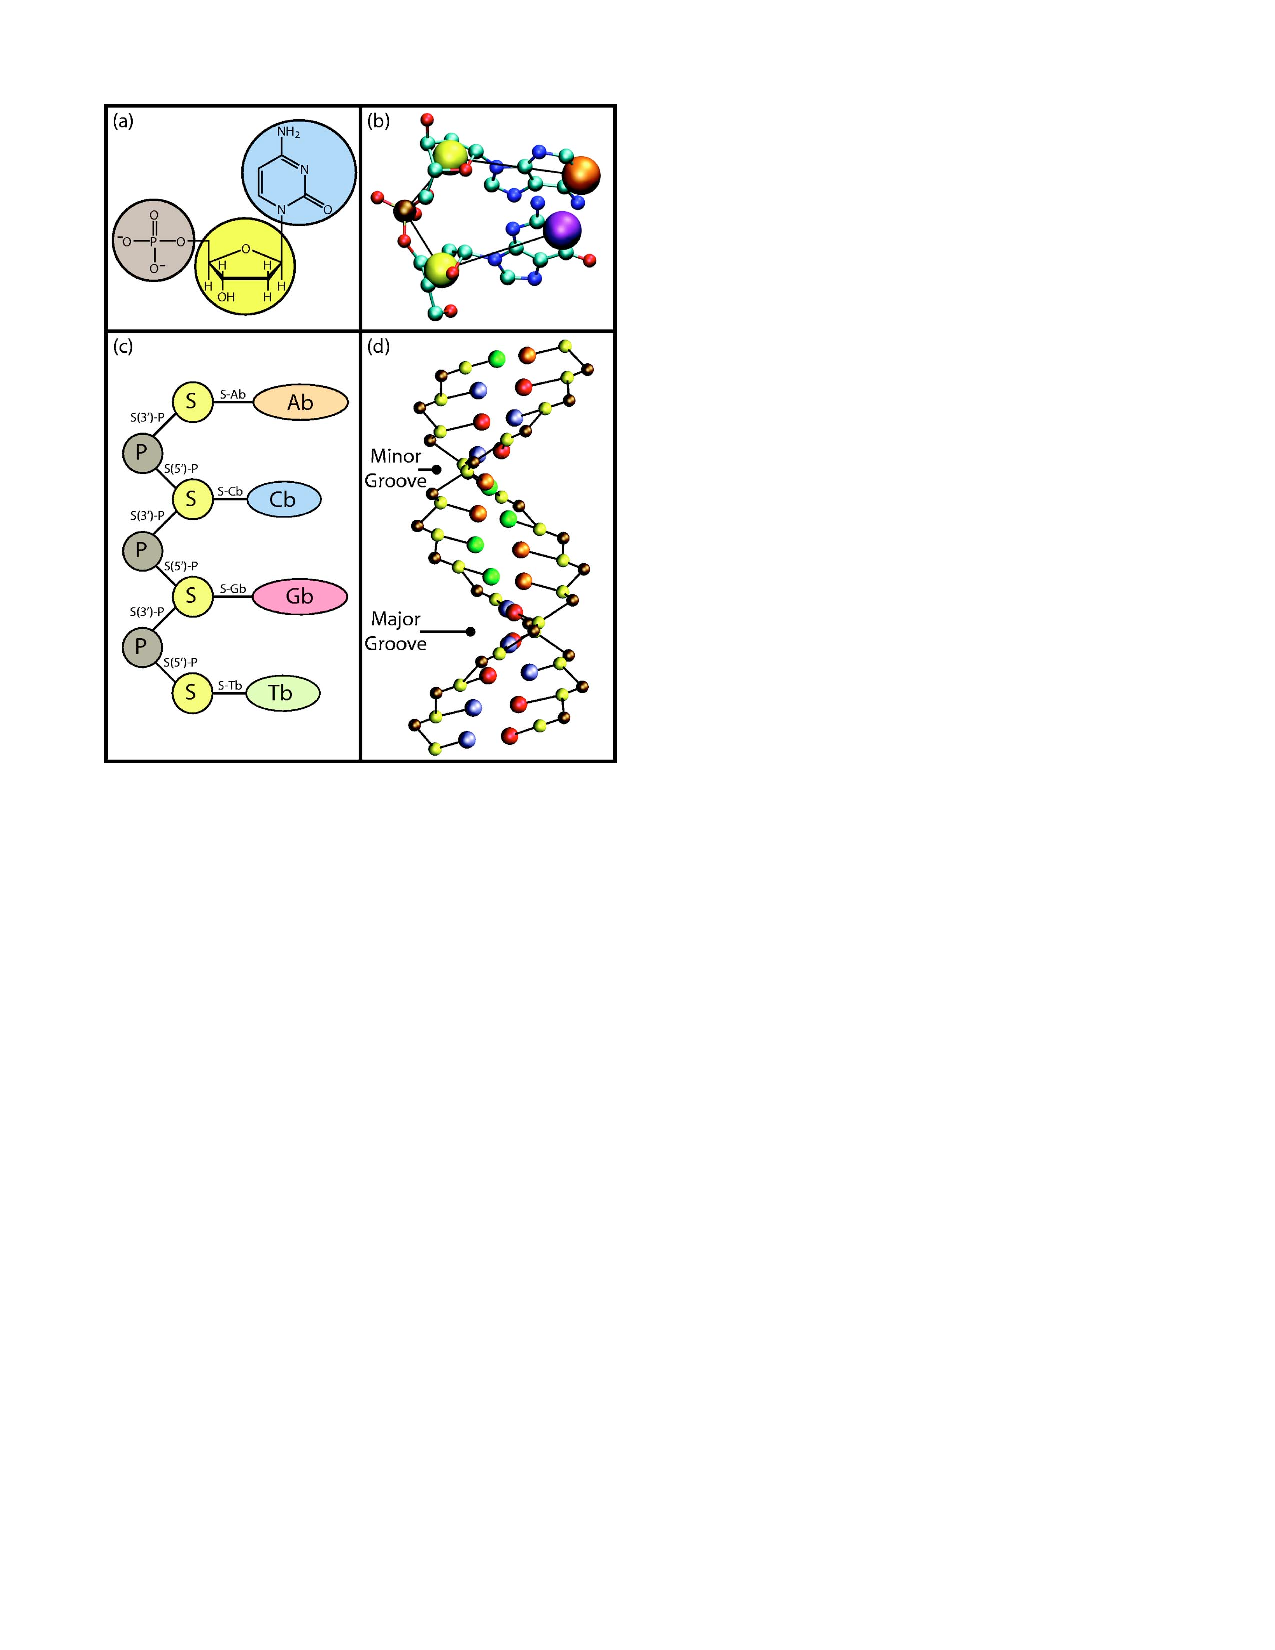
\includegraphics{images/schematic_structure_knotts}
\caption{The schematic structure of the model for B-DNA, from Knotts \etal \cite{knotts2007coarse}. Note the placing of the three sites per nucleus relative to the original atomic structure in the upper right panel.}
\label{schematic_knotts}
\end{center}
\end{figure}

\begin{figure}[h]
\begin{center}
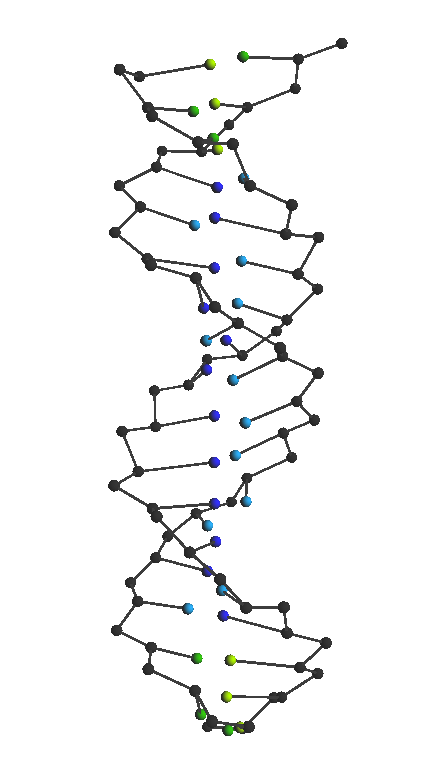
\includegraphics[width=5cm]{images/methods_dnaStructure1} 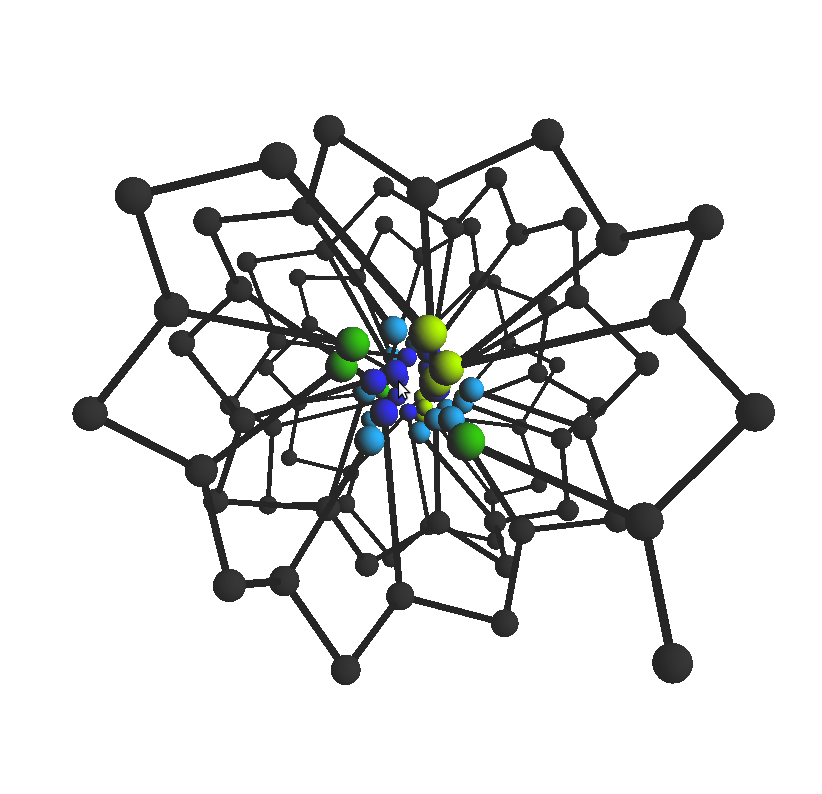
\includegraphics[width=7cm]{images/methods_dnaStructure2}
\end{center}\caption{Side- and top view of the dsDNA structure in our implemented model. The major and minor groove structure in the double helix is clearly visible; as is the screw symmetry from the top view.}
\label{methods_dnaStructure}\end{figure}



